\subsection{BioPlex systematic AP-MS: co-complex check against the IntAct null}
\label{sec:bioplex}
The IntAct audit found no curated physical edge among the 21 AND-gate antigen
pairs, but curated resources can miss complexes that were never assayed at
small scale. BioPlex provides the orthogonal check: systematic affinity
purification--mass spectrometry networks over thousands of baits in two cell
lines (HEK293T 10K and HCT116 5.5K, Dec 2019 releases; @N293EDGES@ and
@NHCTEDGES@ bait--prey edges). The limitation is complementary: a pair is
testable only when both antigens are expressed and detected in the cell line,
so BioPlex can confirm but not exhaustively exclude cis-complexes in
tumor-lineage contexts.

\paragraph{Calibration gate.} Pre-registered gates PASSED: (G1) PSMA1
recovers proteasome beta-subunit partners in both networks (observed
@GATEONE@); (G2) POLR2A recovers at least one Pol~II subunit partner in
293T (observed @GATETWO@); (G3) at least three of four CAR-T reference
targets are detected in 293T (observed @GATETHREE@).

\paragraph{Antigen-pair co-complex test.} Of the 21 antigen pairs,
@TEST293@ are testable in 293T and @TESTHCT@ in HCT116 (both antigens
detected). Observed co-precipitation edges: @EDGES293@ in 293T and
@EDGESHCT@ in HCT116. CA9 and CLDN6 are undetected in both cell lines and
CLDN18 is undetected in HCT116, so pairs involving them remain untestable at
systematic scale. @H1VERDICT@

\paragraph{Detection and degree bias.} Gated genes are detected at higher
rates than background in both networks (@PRES293@ versus @PRESB293@ in 293T,
Fisher $p=@PPRES293@$; @PRESHCT@ versus @PRESBHCT@ in HCT116, $p=@PPRESHCT@$),
so the gated set is well covered where it matters. Among detected genes,
however, AP-MS degree does NOT differ (medians @DEG293@ vs @DEGB293@ in 293T,
$p=@PDEG293@$; @DEGHCT@ vs @DEGBHCT@ in HCT116, $p=@PDEGHCT@$). @H2VERDICT@

\paragraph{Cross-resource concordance.} Restricting to universe--universe
pairs, BioPlex yields @BPEITHER@ edges in either network (@BPBOTH@ reproduced
in both; cross-network Jaccard @JACC@). All @BPINTACT@ BioPlex-either edges
are contained in the IntAct curated physical set (@INTACTN@ universe edges);
IntAct curates the BioPlex screens, so containment is expected by provenance
and serves as a mapping-validation anchor rather than independent evidence.
The @INTACTONLY@ IntAct-only edges are small-scale curated evidence not
reproduced at systematic AP-MS scale in these two cell lines.

\begin{figure}[t]
\centering
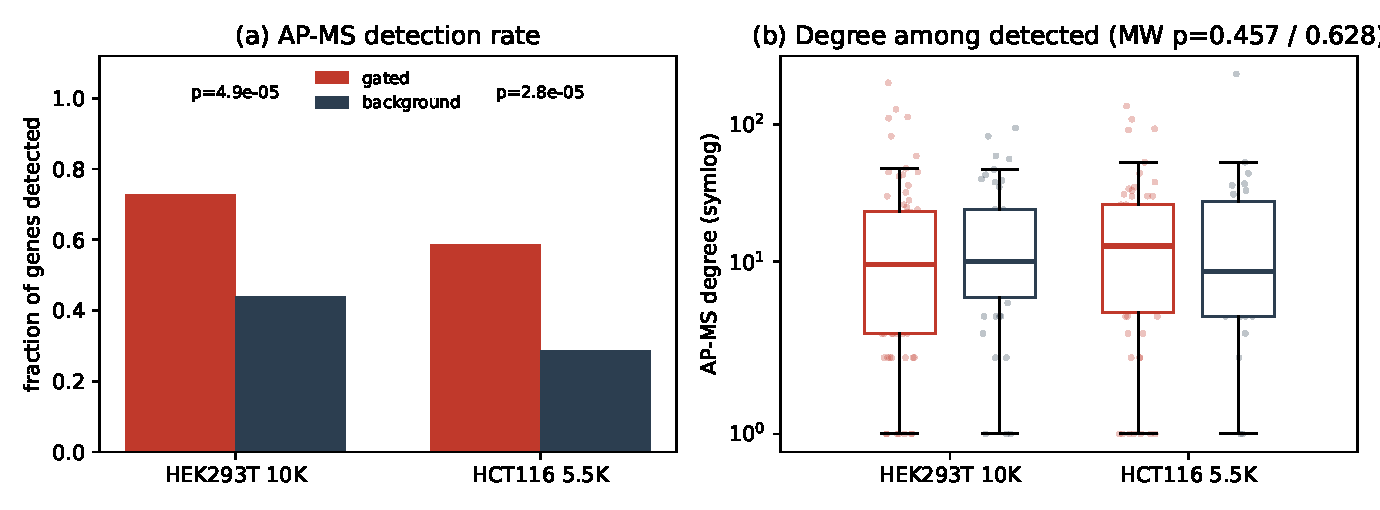
\includegraphics[width=\linewidth]{bioplex_fig.pdf}
\caption{BioPlex systematic AP-MS audit. (a) Detection rate of gated versus
background genes in the two networks. (b) AP-MS degree among detected genes
(symlog axis; boxes show median and quartiles).}
\label{fig:bioplex}
\end{figure}
